\documentclass{article}

\usepackage[utf8]{inputenc}
\usepackage[english]{babel}
\usepackage{geometry}
\usepackage{graphicx} % Required for inserting images
\usepackage{hyperref}
\usepackage{todonotes}
\usepackage{comment}
\usepackage{blindtext}
\usepackage{tikz} \usetikzlibrary{positioning, shadows.blur, shapes.misc}
\usepackage{pgfplots} \pgfplotsset{compat=1.18}
\usepackage{color} % colors
\usepackage{xcolor} % colors
\usepackage{listings} % code listings
\usepackage{amsmath} % equations
\usepackage{colortbl} % coloring the table cell
\usepackage{multirow}
\usepackage{enumitem} % for roman enumeration
% \usepackage{pxfonts} % bold keywords
% \usepackage{xurl} % url in more lines
% \usepackage{tabularx} % fixed columns
% \usepackage{pdfpages} % attach a pdf
% \urlstyle{same} % url has different font to text
\usepackage{longtable} % table in more than 1 page
% \usepackage[autostyle]{csquotes}
% \usepackage{wrapfig} % wrapping figure
\usepackage{placeins} % text after image: \FloatBarrier 
% \usepackage{caption} % removes the "Figure 1" from the cption



\definecolor{grey}{RGB}{175, 175, 175}
\definecolor{green}{RGB}{0, 150, 0}
\definecolor{purple}{RGB}{148,0,211}
\definecolor{blue}{RGB}{0,0,255}
\definecolor{lightblue}{RGB}{246, 249, 255}


\lstdefinestyle{MatLab}{language=MatLab,
  %
  backgroundcolor=\color{lightblue},
  %
  basicstyle=\ttfamily, 
  %
  keywordstyle=\bfseries\color{purple},
  %
  commentstyle=\itshape\small\color{blue},
  %
  stringstyle=\color{green},
  % side numbers
  numberstyle=\tiny\color{grey},
  % 
  belowskip=3mm,
  breakatwhitespace=true,
  breaklines=true,
  classoffset=0,
  columns=flexible,
  framexleftmargin=0.25em,
  frameshape={}{y}{}{}, % to remove to vertical lines on left, set `frameshape={}{}{}{}`
  numbers=left, % if you want line numbers, set `numbers=left`
  showstringspaces=false,
  tabsize=3,
  xleftmargin = 1.5em,
  morekeywords = {nullptr, cout, cin}
}



\usepackage[utf8]{inputenc}
\usepackage[english]{babel}
% sheet size
\usepackage{geometry} \geometry{a4paper, top=4.5cm, bottom=4.5cm, left=4cm, right=4cm} % heightrounded, bindingoffset=5mm}
\usepackage{graphicx} % Required for inserting images
\usepackage{hyperref}
\usepackage{todonotes}
\usepackage{comment}
\usepackage{blindtext}
\usepackage{tikz}\usetikzlibrary{positioning, shadows.blur, shapes.misc}
\usepackage{pgfplots}\pgfplotsset{compat=1.18}
\usepackage{color} % colors
\usepackage{listings} % code listings
\usepackage{amsmath} % equations
% \usepackage{enumitem} % for roman enumeration
% \usepackage{pxfonts} % bold keywords
% \usepackage{xurl} % url in more lines
% \usepackage{tabularx} % fixed columns
% \usepackage{pdfpages} % attach a pdf
% \urlstyle{same} % url has different font to text
% \usepackage{longtable} % table in more than 1 page
% \usepackage[autostyle]{csquotes}
% \usepackage{wrapfig} % wrapping figure
% \usepackage{placeins} % text after image: \FloatBarrier 
% \usepackage{caption} % removes the "Figure 1" from the cption

\setuptodonotes{fancyline, color=green!40}

% Changes title of ToC
\addto\captionsenglish{ %
  \renewcommand{\contentsname}%
    {Index}%
}

% \setlist[itemize]{label=$\diamond$} % alwais diamond-item list


% index of images
% \usepackage{array}
% \graphicspath{ {figures/} }


% changes from "Listing 1" to "Code snippet"
\addto\captionsitalian{%
\renewcommand{\lstlistingname}{Code snippet}}

% changes from "Listings" to "Code snippets"
\addto\captionsitalian{% 
\renewcommand{\lstlistlistingname}{Code snippets}}



% Line-spacing
% \usepackage{setspace} 
% \onehalfspacing % line-spacing 1.5
% \doublespacing % line-spacing 2

\title{\vspace{160px} \textbf{\huge{Analysis and simulation of a digital transmission system}}}
\author{\Large{\href{https://github.com/imAlessas}{Alessandro Trigolo}}}
\date{2023/2024}


\def\analysis{1}
\def\simulation{1}




\begin{document}

\maketitle
\thispagestyle{empty}
\newpage

\tableofcontents \newpage

\listoftodos \newpage






\setcounter{secnumdepth}{0}
\section{Introduction}
\todo{Finish introduction}
This document analyses and simulates the behavior of a digital transmission system. The document is split into two main parts:

\begin{enumerate}[label=\roman*]
    \item \textbf{Analysis.} \hyperref[raw-results]{\texttt{Raw results}} section
    % 
    \item \textbf{Simulation.}
\end{enumerate}



You can find the full project at \texttt{\href{https://github.com/imAlessas/transmission-simulation.git}{imAlessas/transmission-simulation.git}}.

\subsection{General schematic}
The full schematic - containing every step - of a transmission system is presented in figure \ref{fig:transmission_diagram}. Before exploring the mathematical background hidden between the steps, it is crucial to understand what every phase of the system means.

\begin{itemize}
    \renewcommand{\labelitemi}{$\diamond$}
    \item \textsl{Source.} The source device is whichever device is sending a signal; it could be a television, a computer, a smartphone, or anything else.
    % 
    \item \textsl{Formatting Device.} The formatting device's task is to translate the information from analogic to digital which translates into sampling the continuous analogic signal and creating a discrete digital signal that can be transmitted through digital devices.
    % 
    \item \textsl{Source Coding.} The source coding goal is lossless data compression. Sure enough, through the Shannon-Fano source coding, the symbols transmitted are encoded to reduce the average codeword length.
    % 
    \item \textsl{Channel Coding.} 
    % 
    \item \textsl{Interleaving.} The interleaver is needed to transform package errors into independent errors. This is achieved by changing the ordering of the symbols that will be transmitted.
    % 
    \item \textsl{Scrambling.} The scrambling procedure helps with the synchronization between the two devices and improves the security of the transmission. This is achieved by adding a \textit{pseudo-random sequence} to the symbols before the transmission.
    % 
    \item \textsl{Modulation.} The modulation process' goal is to match the spectrum of the transmitted signal with the transmission channel bandwidth making the signal more noise-immune and increasing the data-transfer rate; these operations are performed by the modulator. There are different types of modulation, the one utilized in this project is the \textsl{Binary Phase Shift Keying}, which is one of the most effective modulations against noise. 
    % 
    % 
    \begin{figure}[b!]
    \centering
    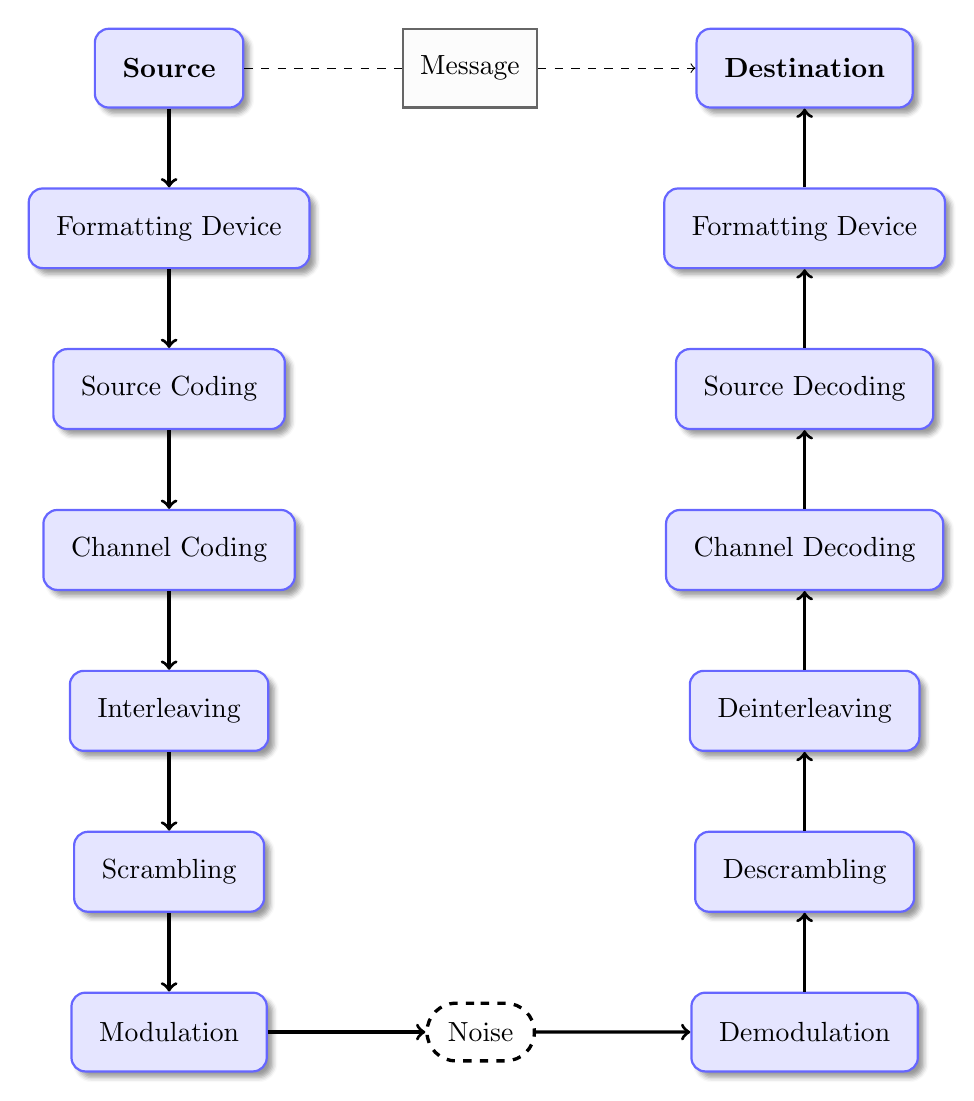
\begin{tikzpicture}[
        Step/.style = {rectangle, rounded corners = 5, inner sep = 10, draw = blue!60, fill = blue!10, thick, blur shadow, minimum size = 1cm},
        % 
        Noise/.style = {rounded rectangle, inner sep = 7, draw = black, dashed, very thick},
        % 
        Message/.style = {rectangle, draw = black!60, fill = black!1, thick, minimum width = 1.7cm, minimum height = 1cm },
    ]
        % Source
        \node[Step] (Source) {\textbf{Source}};
        \node[Step] (FormDevSou) [below = of Source] {Formatting Device};
        \node[Step] (SourceCoding) [below = of FormDevSou] {Source Coding};
        \node[Step] (ChanCod) [below = of SourceCoding] {Channel Coding};
        \node[Step] (Interleaving) [below = of ChanCod] {Interleaving};
        \node[Step] (Scrambling) [below = of Interleaving] {Scrambling};
        \node[Step] (Modulation) [below = of Scrambling] {Modulation};

        % Noise
        \node[Noise] (Noise) [right = 2cm of Modulation] {Noise};

        % Message
        \node[Message] (Message) [right = 2cm of Source] {Message};

        % Destination
        \node[Step] (Destination) [right = 2cm of Message] {\textbf{Destination}};
        \node[Step] (FormDevDest) [below = of Destination] {Formatting Device};
        \node[Step] (SourceDec) [below = of FormDevDest] {Source Decoding};
        \node[Step] (ChanDec) [below = of SourceDec] {Channel Decoding};
        \node[Step] (Deinterleaving) [below = of ChanDec] {Deinterleaving};
        \node[Step] (Descrambling) [below = of Deinterleaving] {Descrambling};
        \node[Step] (Demodulation) [below = of Descrambling] {Demodulation};
        



        % Arrow Message
        \draw[-, dashed] (Source) to node[]{} (Message);
        \draw[->, dashed] (Message) to node[]{} (Destination);


        % Arrows source
        \draw[->, very thick] (Source) to node[]{} (FormDevSou);
        \draw[->, very thick] (FormDevSou) to node[]{} (SourceCoding);
        \draw[->, very thick] (SourceCoding) to node[]{} (ChanCod);
        \draw[->, very thick] (ChanCod) to node[]{} (Interleaving);
        \draw[->, very thick] (Interleaving) to node[]{} (Scrambling);
        \draw[->, very thick] (Scrambling) to node[]{} (Modulation);

        % Noise
        \draw[->, very thick] (Modulation) to node[]{} (Noise);
        \draw[->, very thick] (Noise) to node[]{} (Demodulation);

        % Arrows destination
        \draw[->, very thick] (Demodulation) to node[]{} (Descrambling);
        \draw[->, very thick] (Descrambling) to node[]{} (Deinterleaving);
        \draw[->, very thick] (Deinterleaving) to node[]{} (ChanDec);
        \draw[->, very thick] (ChanDec) to node[]{} (SourceDec);
        \draw[->, very thick] (SourceDec) to node[]{} (FormDevDest);
        \draw[->, very thick] (FormDevDest) to node[]{} (Destination);

    \end{tikzpicture}
    \caption{The diagram of the digital information transmission system.}
    \label{fig:transmission_diagram}
\end{figure}
    % 
    % 
    \item \textsl{Noise.} The noise is a crucial obstacle to overcome to have a successful transmission; the noise is the main reason for a wrongly transmitted symbol. There are different types of noise, some of them are generated by other transmissions, others are due to the physical medium and others are caused by the intermediate devices between the transmission. Nevertheless, in every transmission, there will be the \textsl{Gaussiam White Noise} which is a thermal noise caused by the Big Bang.
    % 
    \item \textsl{Demodulation.} In this phase the demodulator device, after receiving the disturbed signal, will try to detect the signal to regenerate the original one. Sometimes the noise energy will be stronger than the signal energy generating errors that will be corrected in the next steps.
    % 
    \item \textsl{Descrambling.} The descrambling procedure is the opposite of the scrambling. The added \textit{pseudo-random sequence}, after the reception is subtracted by the descrambler.
    % 
    \item \textsl{Deinterleaving.} The deinterleaver reorders the transmitted symbols in the opposite way that the interleaver did. In such a way the \textit{burst} errors that occurred during the transmission will become single errors that can be easily recovered.
    % 
    \item \textsl{Channel Decoding.} 
    % 
    \item \textsl{Source Decoding.} The source decoding procedure decompresses the received data into the original symbols. This is achieved by one of the source coding properties: symbols are easily detected because there are no shorter codes at the beginning of longer codes.
    % 
    \item \textsl{Formatting Device.} During the transmission this device converts the signal from analogic to digital, during the reception of the signal the formatting device translates the discrete digital signal into a continuous analogic signal. 
    % 
    \item \textsl{Destination.} The destination device is whichever device will receive the signal. Likewise the source one, the destination device could be a satellite, a smartphone, a server, or anything else.
\end{itemize}

\subsection{Initial parameters}
The parameters used in this project have been assigned in a datasheet and are reported in the following list:
\vspace{-5px}
\begin{itemize}
    \renewcommand{\labelitemi}{$\cdot$}
    \setlength{\itemsep}{-2px}
    \item \textsl{Symbol duration}: 60 ns, also called $\tau$;
    \item \textsl{SNR}: 8.1 dB;
    \item \textsl{Source code}: Shannon-Fano coding;
    \item \textsl{Error correction code}: cyclic coding with codeword length \textit{m = 31} and generator polynomial $ z^5 \oplus z^2 \oplus 1$;
    \item \textsl{Carrier frequency}: 2.5 GHz;
    \item \textsl{Modulation}: Binary Amplitude Shift Keying (BPSK) with the phase shift of $\pi$.
\end{itemize}

\noindent In addition, the source data (alphabet) and the symbols' respective probabilities are summarized in the following table.

\begin{table}[h!]
    \centering
    \begin{tabular}{|c|c|}
        \hline
        \multicolumn{2}{|c|}{\texttt{Source 7}} \\\hline\hline
        $ a_1 $ & 0.11 \\
        $ a_2 $ & 0.07 \\
        $ a_3 $ & 0.09 \\
        $ a_4 $ & 0.01 \\
        $ a_5 $ & 0.06 \\
        $ a_6 $ & 0.06 \\
        $ a_7 $ & 0.13 \\
        $ a_8 $ & 0.14 \\
        $ a_9 $ & 0.13 \\
        $ a_{10} $ & 0.05 \\
        $ a_{11} $ & 0.11 \\
        $ a_{12} $ & 0.04 \\\hline
    \end{tabular}
    \label{tab:source7}
\end{table}

\noindent Afterwards the parameters have been transcripted in the MATLAB program, as shown in the following snippet. 

\begin{lstlisting}
% source number 7
ALPHABET = [1, 2, 3, 4, 5, 6, 7, 8, 9, 10, 11, 12];
PROBABILITY_VECTOR = [11, 7, 9, 1, 6, 6, 13, 14, 13, 5, 11, 4]/100;

TAU = 60e-9; % symbol duration time, [s]
SNR = 8.1; % Signal-to-Noise-Ration, [dB]
% Source Code: Shannon-Fano
% Error correction code: Cyclic
CODEWORD_LENGTH = 31; % m
% 
F_0 = 2.5e+9; % carrier frequency [Hz]
% Modulation: BPSK
PHASE_SHIFT = pi; % [rad]
U = 1; % amplitude BPSK signal [V]

transmitted_symbol_number = 20;
\end{lstlisting}





\setcounter{secnumdepth}{1}



\if\analysis1
    \newpage \part{Analysis}

    \section{Source data}

The source data analysis provides a general overview of how the data are generated and how this will impact the encoding scheme. Specifically, the source data analysis is achieved by calculating two important values: the source entropy and the redundancy coefficient.

\subsection{Source entropy}

The source entropy $H$ and the maximum source entropy $H_{\max}$. The entropy of a sequence of symbols is a number that summarizes the randomness of the selection of the symbols in the source sequence. The more uncertain the symbols are, the higher the entropy is and the higher the information the symbols carry. The ideal entropy is when the source symbols are \texttt{1 0 1 0 1 0 \dots} while the worst entropy is when all the symbols are \texttt{1} or \texttt{0}. Given a sequence $S$ of $N$ symbols, where each of them has its probability $P_i$ to occur, the entropy of the sequence is:

\begin{equation*}
    H(S) = - \sum_{i = 1}^{N}\,P_i \log_2 P_i
\end{equation*}

\noindent The entropy calculation can be simply achieved with the following MATLAB code. The only thing to note is that P is the probability vector that assigns to every symbol of the alphabet its probability. 

\begin{lstlisting}  
    % sum(V .* log2(V))
    H = - dot(PROBABILITY_VECTOR, log2(PROBABILITY_VECTOR));
\end{lstlisting}

\noindent Secondly, in order to calculate the maximum entropy $H_{\max}$, two conditions have to be met: all of the symbols have the same probability $P_i = \frac{1}{N}$ and, of course, they do not correlate one another. Consequently:

\begin{equation*}
    H_{\max}(S) = - \sum_{i = 1}^{N}\,\frac{1}{N} \log_2 \frac{1}{N} = \frac{1}{N} \sum_{i = 1}^{N}\, \log_2 N = \log_2N
\end{equation*}

\noindent Also in this case the MATLAB script to calculate the maximum entropy is trivial.

\begin{lstlisting}
    % Number of symbols in the alphabet
    N  = length(PROBABILITY_VECTOR);

    % Maximum source entropy
    H_max = log2(N);
\end{lstlisting}

\noindent By running the scripts, the value obtained are $H = 3.3995$ while $H_{\max} = 3.5850$. Reasonably $H < H_{\max}$ because the given probabilities in the datasheet weren't equal to each other.

% 
\subsection{Redundancy coefficient}

The redundancy coefficient $\rho$ summarizes in a number how much additional information is present inside the sequence. Essentially, the lower the redundancy coefficient is, the better, because it means that the source entropy is very high. Mathematically, the coefficient $\rho$ can be obtained as follows:

\begin{equation*}
    \rho = 1 - \frac{H}{H_{\max}}(S)    
\end{equation*}

\noindent which translates into the following code snippet:

\begin{lstlisting}
    % Calculate the redundancy coefficient 'rho'
    source_redoundancy = 1 - H/H_max;
\end{lstlisting}

\noindent Expectedly, the redundancy coefficient is not zero because $H<H_{\max}$: by running the script, $\rho = 0.0517$.



 % Task 2

    \vspace{40px} \section{Source encoding} \label{source-encoding}
The source coding analysis provides the necessary tools to evaluate the source coding algorithms for efficient data representation and compression. In this case, the analysis calculates and uses different values to provide a better understanding of the efficiency of the Shannon-Fano source coding. Particularly the values that will be analyzed are the average codeword length $\overline{m}$, the probability of \texttt{1} and \texttt{0} ($P_1$ and $P_0$), the binary entropy $H_{bin}$, the source data generation rate $R$ and the compression ratio $K$.


\subsection{Shannon-Fano algorithm}
Before calculating the values it is important to encode the symbols of the alphabet through the Shannon-Fano algorithm. A brief recursive description of it is reported below.
\begin{enumerate}
    \item Sort the symbol of the alphabet by descending probability;
    \item Divide the sets of symbols into two continuous subsets with the same probability (or the lowest difference between the two);
    \item Assign to one subset the symbol 1 and the other 0;
    \item Repeat until every subset consists of one symbol;
    \item Read the codeword from left to right.
\end{enumerate} 

\noindent By applying the Shannon-Fano algorithm to the given source, the result should be the following.

\begin{table}[h]
    \centering
    \begin{tabular}{|c|c|c c c c c|c|c|c|c|}
        \hline
        \texttt{S} & \texttt{P} & \multicolumn{5}{c|}{Shannon-Fano} & \texttt{Code} & $m$ & $m_0$ & $m_1$ \\ \hline\hline
        $a_8$    & 0.14 & \cellcolor{teal!25} & \cellcolor{cyan!15} & 1 &  &  & \texttt{111} & 3 & 0 & 3\\
        $a_7$    & 0.13 & \cellcolor{teal!25} & \multirow[vpos]{-2}{*}{\cellcolor{cyan!15}1} & 0 &  &  & \texttt{110} & 3 & 1 & 2\\
        $a_9$    & 0.13 & \cellcolor{teal!25} & \cellcolor{cyan!20} & 1 &  &  & \texttt{101} & 3 & 1 & 2\\
        $a_1$    & 0.11 & \multirow[vpos]{-4}{*}{\cellcolor{teal!25}1} & \multirow[vpos]{-2}{*}{\cellcolor{cyan!20}1} & 0 &  &  & \texttt{100} & 3 & 2 & 1\\
        $a_{11}$ & 0.11 & \cellcolor{green!25} & \cellcolor{lime!25} & 1 &  &  & \texttt{011} & 3 & 1 & 2\\
        $a_3$    & 0.09 & \cellcolor{green!25} & \cellcolor{lime!25} & \cellcolor{lime!15} & 1 &  & \texttt{0101} & 4 & 2 & 2\\
        $a_2$    & 0.07 & \cellcolor{green!25} & \multirow[vpos]{-3}{*}{\cellcolor{lime!25}1} & \multirow[vpos]{-2}{*}{\cellcolor{lime!15}0} & 0 &  & \texttt{0100} & 4 & 3 & 1\\
        $a_5$    & 0.06 & \cellcolor{green!25} & \cellcolor{lime!35} & \cellcolor{yellow!25} & 1 &  & \texttt{0011} & 4 & 2 & 2\\
        $a_6$    & 0.06 & \cellcolor{green!25} & \cellcolor{lime!35} & \multirow[vpos]{-2}{*}{\cellcolor{yellow!25}1} & 0 &  & \texttt{0010} & 4 & 3 & 1\\
        $a_{10}$ & 0.05 & \cellcolor{green!25} & \cellcolor{lime!35} & \cellcolor{yellow!35} & 1 &  & \texttt{0001} & 4 & 3 & 1\\
        $a_{12}$ & 0.04 & \cellcolor{green!25} & \cellcolor{lime!35} & \cellcolor{yellow!35} & \cellcolor{orange!15} & 1 & \texttt{00001} & 5 & 4 & 1\\
        $a_4$    & 0.01 & \multirow[vpos]{-8}{*}{\cellcolor{green!25}0} & \multirow[vpos]{-5}{*}{\cellcolor{lime!35}0} & \multirow[vpos]{-3}{*}{\cellcolor{yellow!35}0} & \multirow[vpos]{-2}{*}{\cellcolor{orange!15}0} & 0 & \texttt{00000} & 5 & 5 & 0\\
        \hline
    \end{tabular}
    \label{tab:shannon-fano}
\end{table}

\FloatBarrier \noindent After computing the Shannon-Fano algorithm to the given source, the results should be inserted into the MATLAB program, as follows.

\begin{lstlisting}
% Probability vector sorted from highest to lowest
P = sort(PROBABILITY_VECTOR, 'descend');


% Values obtained with Shannon-Fano code algorithm

% Symbols codeword length
m = [3, 3, 3, 3, 3, 4, 4, 4, 4, 4, 5, 5]; 

% Number of 0s inside the symbols codeword
m_0 = [0, 1, 1, 2, 1, 2, 3, 2, 3, 3, 4, 5];

% Number of 1s inside the symbols codeword
m_1 = [3, 2, 2, 1, 2, 2, 1, 2, 1, 1, 1, 0];
\end{lstlisting}


\subsection{Binary entropy}
At this point, there is all the needed information to calculate the required data for the analysis. First of all, to calculate the average codeword length $\overline{m}$ of $N$ symbols, the following formula should be computed:

\begin{equation*}
    \overline{m} = \sum_{i = 1}^N\,m_i \cdot P_i 
\end{equation*}

\noindent Additionally, to calculate $P_0$ and $P_1$, it is necessary to calculate also the average number of 0 and 1 symbols. The formula is the same as for the average codeword length:

\begin{equation*}
    \overline{m_0} = \sum_{i = 1}^N\,m_{0_i} \cdot P_i 
    \hspace*{40px}
    \overline{m_1} = \sum_{i = 1}^N\,m_{1_i} \cdot P_i
\end{equation*}

\noindent After inserting these formulas in the MATLAB script, the values are $\overline{m} = 3.4300$, $\overline{m_0} = 1.6400$ and $\overline{m_1} = 1.7900$.

\begin{lstlisting}
% Average codeword length
m_average = dot(P, m); 

% Average number of 0 symbols
m_0_average = dot(P, m_0);

% Average number of 1 symbols
m_1_average = dot(P, m_1);
\end{lstlisting}


\noindent Moreover, by dividing the number of 0 or 1 symbols by the average length of the codeword the two probabilities, $P_0$ and $P_1$, can be computed:

\begin{equation*}
    P_0 = \frac{\overline{m_0}}{\overline{m}}
    \hspace*{40px}
    P_1 = \frac{\overline{m_1}}{\overline{m}}
\end{equation*}

\noindent The two probabilities values are $P_0 = 0.4781$ and $P_1 = 0.5219$. Ideally, the probabilities should be $P_0 = P_1 = 0.5$; nonetheless, the two values are still very close to each other. Finally, with the two probability values the binary entropy $H_{bin}$ can be obtained using the following calculation.

\begin{equation*}
    H_{bin}(S) = - P_0\log_2P_0 - P_1\log_2P_1
\end{equation*}

\noindent By running the following MATLAB script, the value of the binary entropy is $H_{bin} = 0.9986$ which is very close to 1. The higher the entropy is, the more uncertainty is associated with every symbol: this means that encoding the initial data with the Shannon-Fano algorithm provides a great value, information-wise.

\begin{lstlisting}
% Probability of 0 symbol
P_0 = m_0_average / m_average; 

% Probability of 1 symbol
P_1 = m_1_average / m_average; 

% Binary source entropy after coding
H_bin = -P_0 * log2(P_0) - P_1 * log2(P_1); 
\end{lstlisting}


\subsection{Data rate and compression ratio}
After encoding the source data with the Shannon-Fano algorithm, it is important to evaluate the source data generation rate $R$, which can be calculated as follows:

\begin{equation*}
    R = \frac{H(S)}{\overline{m}\tau}\text{, where $\tau$ is the symbol duration}
\end{equation*}
 
\noindent The data compression ratio $K$ is important as well: it helps evaluate how much the initial data has been compressed after the source coding. The following formula will help to obtain this value.

\begin{equation*}
    K = \frac{\overline{m}}{H(S)}
\end{equation*}

\noindent After running the MATLAB script displayed below, the data rate $R = 16.519 Mbit/s$ which should be lower than the channel capacity $C_{chan}$ with noise. Moreover, the compression ratio $K = 1.0090$ which is very close to 1, means that the overall compression is low: this is still not a bad result because the overall entropy is increased significantly after the source coding.

\begin{lstlisting}
% Calculate Data Rate
R = H * (m_average * TAU) ^ (-1);

% Calculate Compression Ratio
K = m_average / H;
\end{lstlisting}
 % Task 3

    \vspace{40px} \section{Shannon's theorem condition}

 % Task 4

    \vspace{40px} \section{Error correction}
The error correction analysis is important to understand how powerful and yet dangerous the error correction codes are. In this document, the analysis focuses on the \textsl{cyclic Hamming code} error correction properties even though the conclusions are still valid for the \textsl{group Hamming code} (both systematic and non-systematic). 

Before analyzing the error correction code, it is necessary to properly implement it. The first thing to do is to generate a binary sequence and the encoding and decoding matrix. To do so it has been used the \texttt{cyclgen} function which should be imported from the communication package as follows: \texttt{import communications.*}. These steps are summarized in the code snipped below.

\begin{lstlisting} 
    % generate a sequence of k binary symbols
    binary_sequence =  randi(2, 1, k) - 1;

    % generate decoding and encoding matrix
    [cyclic_decoding_matrix, cyclic_encoding_matrix] = cyclgen(codeword_length, generation_polynomial);

    % reorder the matrixes
    % [6 -> 31, 1 ->]
    reorder = [6:codeword_length, 1:5];

    cyclic_encoding_matrix = cyclic_encoding_matrix (:, reorder); 

    cyclic_decoding_matrix = (cyclic_decoding_matrix (:, reorder))'; 
\end{lstlisting}

\noindent One crucial thing to do is to redefine the associations between the syndrome values and the error position. The vector that is shown below is not random at all but it has been calculated using the algorithm shown in the chapter \ref{hamming-decoding} and the copy-pasted it. This vector is very important because if it is not defined the correction algorithm won't work at all but will increase the error rate.

\begin{lstlisting} 
    % Associates the syndrome to the bit.
    % This vector has been calculated in the hamming_decoding function and copy-pasted here.
    associations = [0 31 30 13 29 26 12 20 28 2 25 4 11 23 19 8 27 21 1 14 24 9 3 5 10 6 22 15 18 17 7 16];
\end{lstlisting} 

\noindent After setting up the error correction algorithm, it is possible to begin the analysis by encoding the codeword and studying the behavior of the cyclic Hamming code. Reasonably, by introducing no errors the decoded codeword is the same as the initial codeword.

\begin{lstlisting} 
    % encode the codeword
    codeword = mod(binary_sequence * cyclic_encoding_matrix, 2);
    initial_codeword = codeword;
    
    % decode without errors
    syndrome_no_error = mod(codeword * cyclic_decoding_matrix, 2);
\end{lstlisting}

\noindent For the next analysis, to properly understand the functioning of the error correction cyclic code, it will be used the following 26-symbols randomly-generated binary sequence:

\begin{center}
    \texttt{1 0 1 0 0 1 0 1 0 1 1 0 1 0 1 0 0 1 1 1 1 0 0 1 1 0}
\end{center}

\noindent The above sequence, after the cyclic hamming encoding will have 31 symbols as follows:
\begin{center}
    \texttt{1 0 1 0 0 1 0 1 0 1 1 0 1 0 1 0 0 1 1 1 1 0 0 1 1 0 }\textcolor{blue}{\texttt{0 0 1 0 0}}
\end{center}

\subsection{One error}
By introducing one error to a random position it is necessary to calculate the decimal syndrome value and then use the \texttt{associations} vector to detect and correct the error. The code snippet presented below sums up the error correction after one error is displayed below.

\begin{lstlisting}
% introduce one error
error_position = randi(31, 1);
codeword(error_position) =~ codeword(error_position);

codeword_one_error = codeword;

% get the error syndrome
syndrome_one_error = mod(codeword_one_error * cyclic_decoding_matrix, 2);

% convert the syndrome into decimal
syndrome_one_error_decimal = bin2dec(num2str(syndrome_one_error));

% get the index of the wrong symbol
wrong_symbol_position = associations(syndrome_one_error_decimal + 1);

% correct the error
codeword_one_error(wrong_symbol_position) = ~codeword_one_error(wrong_symbol_position);
\end{lstlisting}

\noindent By introducing one error in a random position, like position 30, the wrong sequence would be the following:

\begin{center}
    \texttt{1 0 1 0 0 1 0 1 0 1 1 0 1 0 1 0 0 1 1 1 1 0 0 1 1 0 }\textcolor{blue}{\texttt{0 0 }}\textcolor{red}{\texttt{0 }}\textcolor{blue}{\texttt{0 0}}
\end{center}

\noindent Nonetheless the code manages to spot the error using the syndrome value:

\begin{center}
    \texttt{0 0 0 1 0}
\end{center}

\noindent It must be highlighted again the importance of the \texttt{associations} vector because the decimal value of the syndrome is not 30 but it is 2. The vector bonds the decimal value 2 to the position error 30 succesfully managing to perform the error correction:
\begin{center}
    \texttt{1 0 1 0 0 1 0 1 0 1 1 0 1 0 1 0 0 1 1 1 1 0 0 1 1 0 }\textcolor{blue}{\texttt{0 0 1 0 0}}
\end{center}


\subsection{Two errors} \label{two-errors-correction}
By using the below-displayed code, very similar to the previous one, it is possible to introduce a second error to the codeword to analyze the effect of two errors in the codeword. 

\begin{lstlisting}
% introduce second error
error_position = randi(31, 1);
codeword(error_position) =~ codeword(error_position);

codeword_two_errors = codeword;

% get the error syndrome
syndrome_two_errors = mod(codeword_two_errors * cyclic_decoding_matrix, 2);

% convert the syndrome into decimal
syndrome_two_errors_decimal = bin2dec(num2str(syndrome_two_errors));

% get the index of the wrong symbol
wrong_symbol_position = associations(syndrome_two_errors_decimal + 1);

% correct the error
codeword_two_errors(wrong_symbol_position) = ~codeword_two_errors(wrong_symbol_position);
\end{lstlisting}

\noindent By running the code and generating a second error position, like position 11, the codeword becomes the following:

\begin{center}
    \texttt{1 0 1 0 0 1 0 1 0 1 } \textcolor{red}{\texttt{0 }} \texttt{0 1 0 1 0 0 1 1 1 1 0 0 1 1 0 }\textcolor{blue}{\texttt{0 0 }}\textcolor{red}{\texttt{0 }}\textcolor{blue}{\texttt{0 0}}
\end{center}

\noindent Unfortunately in this case the syndrome value will not be helpful:

\begin{center}
    \texttt{0 1 1 1 0}
\end{center}

\noindent which its decimal value is 14, meaning that, using the \texttt{associations} vector, the error position is 19 not corresponding in either the two errors but creating a third error:
\begin{center}
    \texttt{1 0 1 0 0 1 0 1 0 1 } \textcolor{red}{\texttt{0 }} \texttt{0 1 0 1 0 0 1 }\textcolor{red}{\texttt{0 }} \texttt{1 1 0 0 1 1 0 }\textcolor{blue}{\texttt{0 0 }}\textcolor{red}{\texttt{0 }}\textcolor{blue}{\texttt{0 0}}
\end{center}

\noindent For this reason it is important to analyze the probability of two errors occurring in the codeword (see \ref{uncorrectable}): because with the error correction code the two errors not only not be correct but also a third error will be generated in the attempt.

\subsection*{Three erros particoular situation}
If three errors occur in specific positions the algorithm may not even detect the errors because the syndrome is zero. This happens when the three error syndromes cancel each other out. In this case, if the errors are at positions 30 and 11, the critical error position is 14. In this situation, the error syndrome is 0, preventing the algorithm from detecting and correcting any of the three errors. The following code calculates the critical position for any two random error positions using a simple \texttt{brute force} algorithm:

\begin{lstlisting}
    % Three errors experiment
    codeword = initial_codeword;

    % introduce error
    error_position = randi(31, 1)
    codeword(error_position) = ~codeword(error_position);

    % introduce error
    error_position = randi(31, 1)
    codeword(error_position) = ~codeword(error_position);

    critical_position = -1;

    for i = 1 : 31
        % introduce error
        codeword(i) = ~codeword(i);

        % memorize the codeword
        codeword_three_errors = codeword;

        % get the error syndrome
        syndrome_three_errors = mod(codeword_three_errors * cyclic_decoding_matrix, 2);
        
        % convert the syndrome into decimal
        syndrome_three_errors_decimal = bin2dec(num2str(syndrome_three_errors));
        
        % get the index of the wrong symbol
        wrong_symbol_position = associations(syndrome_three_errors_decimal + 1);
        
        if ~wrong_symbol_position
            critical_position = i;
        end
    end
\end{lstlisting}

 % Task 5
    
    \vspace{40px}\section{Bit Error Rate plot}
Another type of analysis that is important to make for the Hamming Code is its overall advantages during the transmission. Particularly, it is important to make a comparison between an encoded transmission (with error correction) and a not encoded transmission. To do so it is important to plot an important graph describing the relationship between the BER in relationship with the SNR value.

To plot such a graph it is necessary to evaluate the Bit Error Rate of the transmission of a random binary sequence with the given modulation (BPSK) for different Signal-to-Noise Ratio. The first thing to do is generate the random sequence and generate the BPSK carrier signal using the given \hyperref[initial-parameters]{initial parameters}:

\begin{lstlisting}
    % Initialize SNR vector
    SNR_vector = 0 : 1/2 : 15; 
        
    % Generation of binary sequence
    N = 1e4; % number of bits to be sent
    N = floor(N / k) * k; % match information block size
    binary_sequence = randi(2, 1, N) - 1;
    
    % Generate carrier signal
    
    % Define the time-step
    delta_t = tau / samples_per_symbol;
    
    % Time intervals for one symbol
    time_intervals = 0: delta_t: tau - delta_t;
    
    % Create the carrier signal
    carrier_signal = sin(2 * pi * f0 * time_intervals); % Carrier signal
    
    % Calculate the energy per symbol
    Eb = dot(carrier_signal, carrier_signal);
\end{lstlisting}

\noindent After creating the carrier signal it is necessary to encode and modulate the randomly generated sequence. To perform the Hamming encoding algorithm it is necessary to create a matrix that will be used in the algorithm. The functioning of the encoding is carefully explained in chapter\,\ref{hamming-encoding}. After Hamming-encoding the sequence the BPSK modulation is performed by transforming the sequence into a Non-Return-to-Zero signal and performing the \textit{Kronecke} multiplication with the carrier signal.

\begin{lstlisting}
    % Hamming encoding
    % Create the matrix for the Hamming-encoding algorithm
    binary_matrix = reshape(binary_sequence, k, N / k)';

    % Hamming-encode the matrix
    hamming_encoded_matrix = hamming_encoding(binary_matrix, codeword_length, k, generation_polynomial); % encode data
    hamming_encoded_matrix = hamming_encoded_matrix';

    % Unwrap the matrix into a single row
    hamming_encoded_sequence = hamming_encoded_matrix(:)';

    % Update the number of bits
    M = N;
    N = length(hamming_encoded_sequence);

    % Modulate the sequence with BPSK
    BPSK_signal = kron(-2 * hamming_encoded_sequence + 1, carrier_signal);
\end{lstlisting}

\noindent Before calculating the different BER values it is necessary to generate the noise power and standard deviation as follows:

\begin{lstlisting}
    % Generate noise power

    % Reversed SNR formula
    EbN0 = 10.^(SNR_vector / 10);
    
    % Obtain noise spectral power density
    N0 = Eb./EbN0;
    
    % Calculate sigma for BPSK
    sigma = sqrt(N0 / 2);  
    
    
    % Prepare the vectors for the for-loop
    BER_no_hamming = 1 : length(SNR_vector);
    BER_with_hamming = 1 : length(SNR_vector);
\end{lstlisting}

\noindent The crucial section of the analysis is presented in the following \texttt{for} loop. First of all the Gaussian White Noise is generated for every entry of the \texttt{SNR\_vector} variable and then added to the BPSK modulated signal. At this point, the detection is performed using the \href{https://github.com/imAlessas/telecom-lab-works/blob/main/reports/lab-4/Trigolo_Report_Lab4.pdf}{\textsl{optimal correlation receiver}} and the BPSK threshold which is zero. Before performing the error correction, the detected sequence is compared with the initial sequence to keep calculating the Bit Error Rate without performing the decoding (\texttt{BER\_no\_hamming}). Secondly, the error correction is performed using the detection algorithm, thoughtfully explained in chapter\,\ref{hamming-decoding}, and then the second BER value is computed (\texttt{BER\_with\_hamming}).

\begin{lstlisting}
    for i = 1 : length(SNR_vector)
        % Calculate the GWN for a specific SNR value
        noise = sigma(i) * randn(1, N * samples_per_symbol);

        % Add the noise
        signal_with_noise = BPSK_signal + noise; % add noise in transmitted channel;


        % Use CORRELATION RECEIVER to detect symbols

        % Slice recieved signal into segments in each column
        sliced_signal_with_noise = reshape(signal_with_noise, samples_per_symbol, N);

        % Detect the signal with the BPSK threshold
        detected_signal = carrier_signal * sliced_signal_with_noise < 0;

        
        errors_number_no_hamming = sum(detected_signal ~= hamming_encoded_sequence);

        % Calculate BER value
        BER_no_hamming(i) = errors_number_no_hamming / N;
        

        % Reshape the sequence into a matrix, every row is a codeword
        detected_sequence_matrix = reshape(detected_signal, codeword_length, N/codeword_length)';
        
        % Perform Hamming decoding
        decoded_data_matrix = hamming_decoding(detected_sequence_matrix, codeword_length, k, generation_polynomial); % encode data
        decoded_data_matrix = decoded_data_matrix';

        % Unwrap the matrix into a sequence
        decoded_data_sequence = decoded_data_matrix(:)'; 

        % Check number of erros
        errors_number_with_hamming = sum (decoded_data_sequence ~= binary_sequence);

        % Calculate BER value
        BER_with_hamming(i) = errors_number_with_hamming/M;
    end
\end{lstlisting}

\noindent All the information to plot the BER curve is known. The following script will provide the plots needed to properly analyze the impact of the cyclic Hamming coding during the noisy transmission. Noticeably, the BER graphics are not linear but should be plotted with the logarithmic scale.

\begin{lstlisting}
    % creates figure and settings
    f = figure(1);
    f.Name = 'Analysis of BER curve';
    f.NumberTitle = 'off';
    f.Position = [450, 100, 700, 600];
    
    % Draw plot without Hamming code
    semilogy(SNR_vector, BER_no_hamming, 'b'), grid on;

    % Draw plot with Hamming code
    hold on, semilogy(SNR_vector, BER_with_hamming, 'r'), hold off;

    % Draw theoretical plot
    hold on, semilogy(SNR_vector, error_propability, 'm'), hold off;

    % Draw SNR project value
    hold on, plot([SNR SNR], [1e-4, 1e-1], 'g--'), hold off;

    
    xlabel('Signal-to-Noise Ratio, [dB]'), ylabel('Bit Error Rate'); % lables
    ylim([1e-4, 1e-1]), xlim([0, 10]); % limits
    legend('Uncoded', 'Coded', 'Theoretical', 'Given SNR value'); % legend
\end{lstlisting}

\noindent By running the MATLAB script the plot obtained is displayed in figure\,\ref{fig:BER-plot}. As expected the red plot decreases faster than the blue plot. This is a reasonable and expected result because the error correction code decreases the error rate by correcting the errors occurring during the transmission. Additionally, the given SNR value is plotted with a dotted green line: the red and the green curves do not meet meaning that the given SNR value, the given modulation technique and the given channel coding algorithm are acceptable and valid to successfully perform a digital transmission. 

\begin{figure}[h]
    \centering
    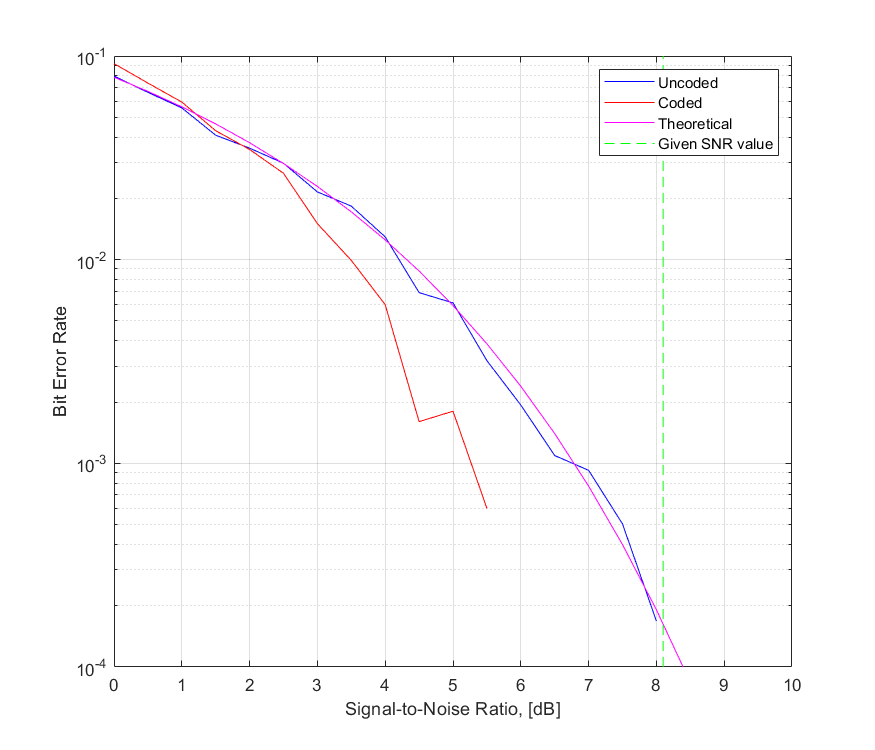
\includegraphics[width = \textwidth]{../res/imgs/BER-plot.png}
    \caption{BER vs SNR plot of a randomly generated sequence.}
    \label{fig:BER-plot}
\end{figure}

One important thing to notice in figure\,\ref{fig:BER-plot} is the beginning of the three plots: the red one is above the blue one meaning that with a low SNR value (meaning that the power of the signal is almost the same as the noise) the error rate of the coded source is higher compared to the uncoded one. This is because when there are 2 or more errors in the codeword the Hamming code is not able to perform the error correction (as explained in the chapter\,\ref{ciclic-coding}) and creates an additional error in the codeword, consequently raising the error probability (or the BER). % Task 6

    \vspace{40px} \section{Modulated signal spectrum}
The spectrum analysis is helpful for a better understanding of the behavior of the BPSK modulation technique. Analyzing the spectrum provides insights into the distribution of signal power across different frequencies. In this section, there will be the analysis an the plots of a periodic \texttt{1010} sequence and a randomly generated sequence.



\subsection{Periodic \texttt{1010} sequence signal}
To analyze and plot the spectrum of a periodic \texttt{1010} sequence signal some important values should be calculated. The $\omega_0$ value, which is the angular carrier frequency, the value, representing the base harmonic frequency and $k$, which is the range in which the spectrum will be calculated. The first two values may be calculated with the following expression:

\begin{equation*}
    \omega_0 = 2\pi f_0 \hspace{30px} \Omega = \frac{\pi}{\tau}
\end{equation*}

\noindent The $k$ range is a range of $n$ indexes around the carrier frequency central index, $k_0 = \omega_0 / \Omega$. These values can be easily obtained by running the below-displayed code snippet.

\begin{lstlisting}
    % anguolar carrier frequency
    omega_0 = 2 * pi * f0; 

    % base harmonic angoular frequency 
    OMEGA = pi / tau; 

    % Carrier frequency central index
    k_0 = omega_0 / OMEGA;

    % Define range of indexes for spectrum
    k = k_0 + (-10 : 10);
\end{lstlisting}

\noindent At this point, the BPSK spectrum can be calculated. To do so it is necessary to calculate the Fourier series coefficient for the BASK\footnote{Which stands for Binary Amplitude Shift Keying} modulation type using the following equation:

\begin{equation*}
    C_{BASK}(k) = j\frac{U}{4} \frac{\sin\left[ \left( k\Omega - \omega_0 \right) \frac{\tau}{2}\right]}{\left( k\Omega - \omega_0 \right) \frac{\tau}{2}}
\end{equation*}

\noindent Now that the BASK coefficients are calculated, the BPSK coefficients are easy to be computed:

\begin{equation*}
    C_{BPSK}(k) = C_{BASK}(k) \left[ e^{+jk\Omega\frac{\tau}{2}} - e^{-jk\Omega\frac{\tau}{2}} \right]
\end{equation*}

\noindent These two complex equations can be computed in MATLAB with the help of the \texttt{sinc} function as follows:

\begin{lstlisting}
    % Phase value of the spectral function
    phase = (k * OMEGA - omega_0) * tau / 2;

    C_BASK = sinc(phase / pi) * U / 4 * 1j; % fourirer series coefficient, BASK

    % BPSK spectrum for periodocal '1' and '0' sequence (...1 0 1 0 1 0 1 0 1 0...)
    C_BPSK = C_BASK .* ( exp(1j * k * OMEGA * tau / 2) -  exp(- 1j * k * OMEGA * tau / 2));
\end{lstlisting}

\noindent After numerically calculating the spectrum, it is very important to plot the result by running the following code snippet.

\begin{lstlisting}
    % creates figure and settings
    f = figure(2);
    f.Name = 'Analysis of BPSK spectrum';
    f.NumberTitle = 'off';
    f.Position = [200, 120, 1200, 600];
    
    % plot 1st result
    stem( k * OMEGA / (2 * pi), abs(C_BPSK), 'b' ), grid on,
    xlabel('Frequency [GHz]'), ylabel('Amplitude, [V]'), title('Amplitude Spectrum of periodic signal')
    ylim([-0.05, 0.35]);
\end{lstlisting}

\noindent By observing the plot displayed in figure\,\ref{fig:periodic-signal-spectrum} it is noticeable that the carrier component in the center of the plot is zero: this is the quirk of the BPSK modulation. Sure enough, the two BASK components subtract at the center of the spectrum but add up in the other cases due to the opposite phase of the formula. 

\begin{figure}[h]
    \centering
    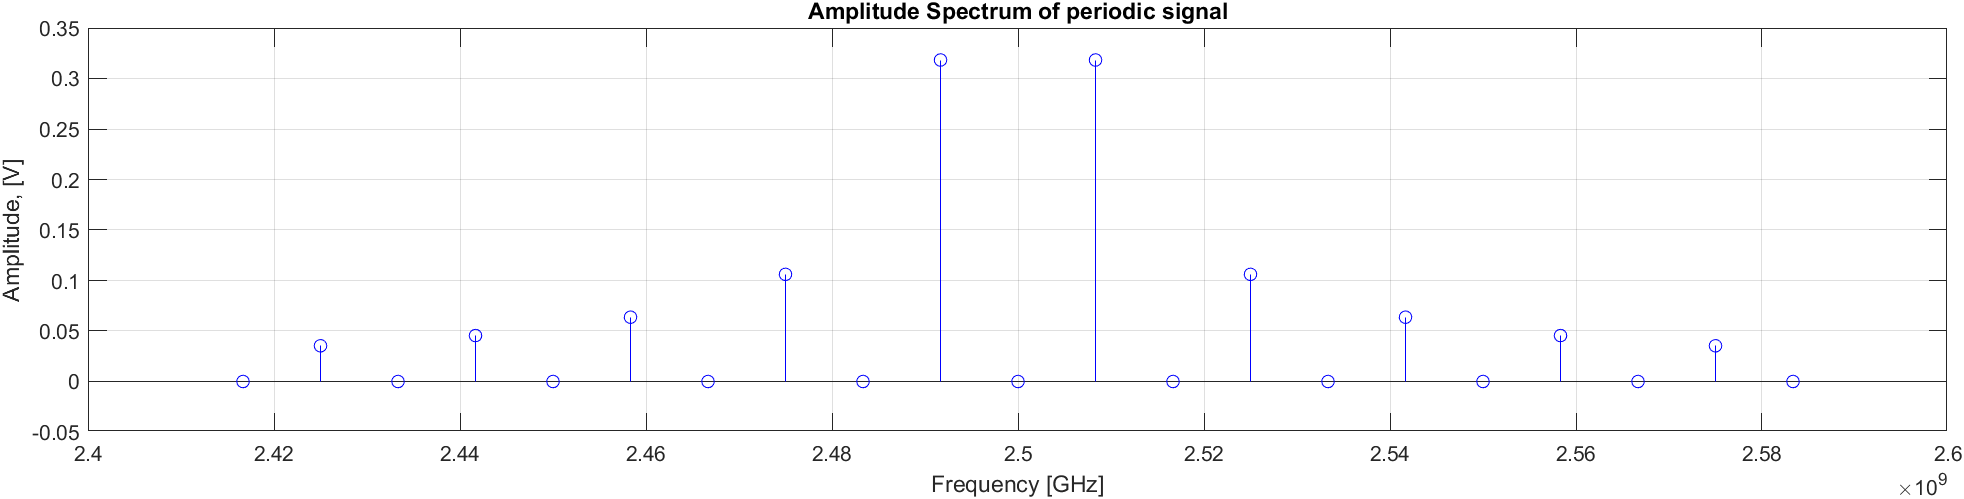
\includegraphics[width = \textwidth]{../res/imgs/periodic-signal-spectrum.png}
    \caption{BPSK periodic signal spectrum.}
    \label{fig:periodic-signal-spectrum}
\end{figure}


\subsection{Random sequence signal}
After plotting and analyzing the spectrum in the case of a periodic signal, it would be important to analyze the spectrum of a random signal as well. To do so it is necessary to get the power spectral density of the BPSK signal, which is double the power spectral density of the BASK modulation:

\begin{equation*}
    G_{BASK}(\omega) = 2\tau|C_{BASK}(\omega)|^2
\end{equation*}

\noindent Consequently the power spectral density of the BPSK signal, called $G_{BPSK}$, can be computed using the following MATLAB script.

\begin{lstlisting}
    % Power Spectral Density (PSD) for random input signal
    omega = ( k(1) : 1/100 : k(end) ) * OMEGA; % angoular frequency 

    phase = (omega - omega_0 ) * tau / 2; % continuous phase 
    S_BASK =  2 * tau * sinc(phase / pi ) * U / 4 * 1j;

    % PSD as a normalized squarred spectral function
    G_BPSK = 1/ tau * abs(S_BASK) .^2;
\end{lstlisting}

\noindent Eventually, as for the spectrum of a periodic signal, the graph can be plotted and generated using the following script.

\begin{lstlisting}
    % creates figure and settings
    f = figure(3);
    f.Name = 'Analysis of BPSK spectrum';
    f.NumberTitle = 'off';
    f.Position = [200, 120, 1200, 600];

    % plot 2nd result
    plot( omega / (2 * pi), G_BPSK, 'b' ), grid on,
    xlabel('Frequency [GHz]'), ylabel('PSD'), title('PSD of random signal')
    ylim([-0.1e-8, 1.6e-8]);
\end{lstlisting}

\noindent The result is that the spectrum of the BPSK signal is extremely high if compared with the BASK and BFSK spectrum due to its particular properties (figure\,\ref{fig:random-signal-spectrum}): the phase shift of $\pi$ doubles the PSD in comparison with the BASK and the BFSK making this modulation technique the most efficient one out of the three.

\begin{figure}[h]
    \centering
    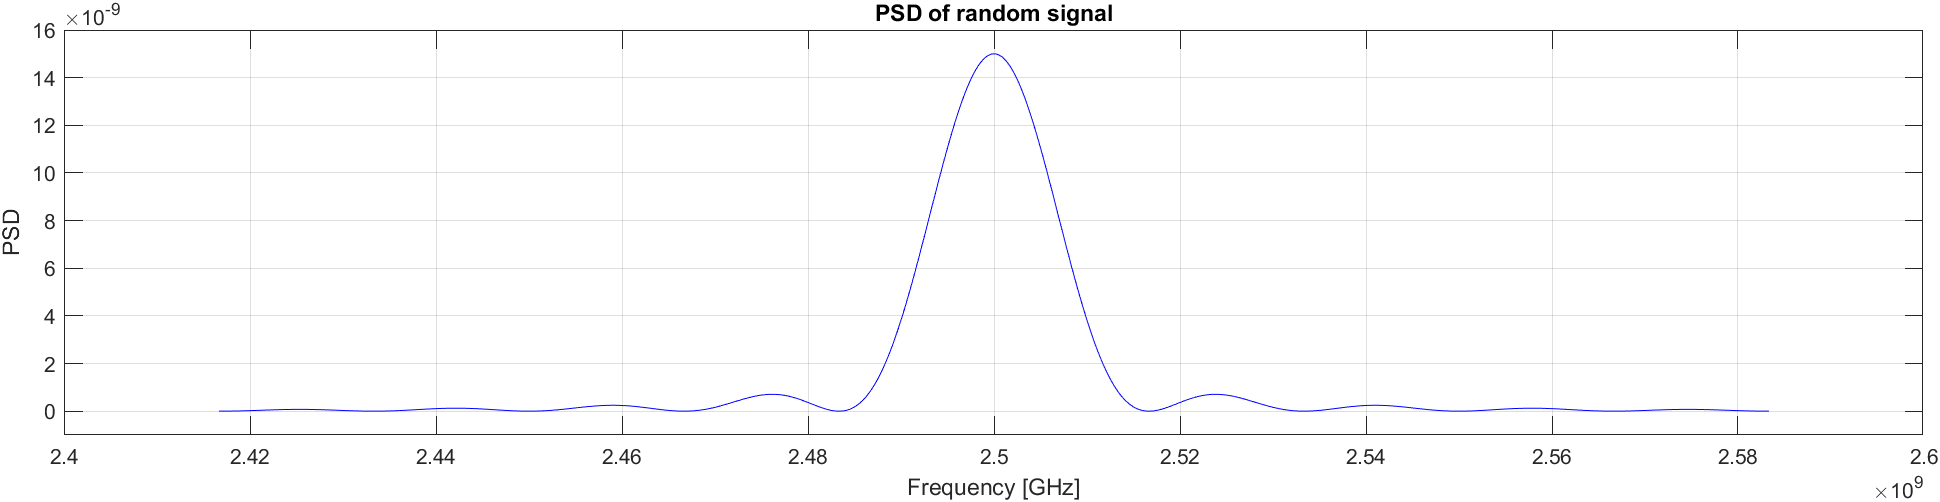
\includegraphics[width = \textwidth]{../res/imgs/random-signal-spectrum.png}
    \caption{BPSK random signal spectrum.}
    \label{fig:random-signal-spectrum}
\end{figure} % Task 7
    
    \vspace{40px} \section{Uncorractable errors} \label{uncorrectable}
The reason for calculating the probability of 2 or more errors occurring in the same codeword has been explained in the previous chapters. The main reason is that the Hamming code is not able to correct 2 or more errors in the codeword: this does not mean that at least one of them is correct but it leads to the creation of another error. Consequently, the probability of an uncorrectable error is strictly bonded to the fact that with that type of error a new error will be almost surely generated by the Hamming code. For this reason, this probability should be as near to zero as possible.

To calculate such a value the mathematical equation below-displayed should be computed:

\begin{equation*}
    P_{\geq2\,err} = 1 - (1 - P_{err})^m - \sum_{i = 1}^g\, C^i_m\,P_{err}^i(1 - P_{err})^{m - i}
\end{equation*}

\noindent In this particular case, $g = 1$ and $C^i_m = m$ so the equation can be simplified as follows:

\begin{equation*}
    P_{\geq2\,err} = 1 - (1 - P_{err})^m - m\,P_{err}^i(1 - P_{err})^{m - 1}
\end{equation*}

\noindent Which translates in the following MATLAB line:

\begin{lstlisting}
    % probability of the case when it is not possible to correct errors with the Hamming code (>= 2 errors)
    P_uncor = 1 - (P_err_comp)^(codeword_length) - codeword_length * P_err * (P_err_comp)^(codeword_length - 1);
\end{lstlisting}

\noindent After running the script the probability of an uncorrectable error $P_{\geq2\,err} = 1.2338\cdot10^{-5}$, which is a low value but, with a high mole of transmitted data there is the possibility to still occur in uncorrectable errors that may lead to an unsuccessful transmission. The probability is still rather low but it is a still possible scenario that should be taken into consideration.

 % Task 8

    \setcounter{secnumdepth}{0}
\vspace{40px}\section{Raw results}\label{raw-results}
\todo{Make a little introduction in the "Raw result" section}

\begin{center}
\renewcommand{\arraystretch}{1.5}
\begin{longtable}{|c|c|c|}
    
    \hline \multicolumn{1}{|c|}{\textbf{Symbol}} & \multicolumn{1}{c|}{\textbf{Description}} & \multicolumn{1}{c|}{\textbf{Value}} \\ \hline 
    \endfirsthead

    \multicolumn{3}{r}%
    {{\small\textit{\dots continued from previous page}}} \\
    \hline \multicolumn{1}{|c|}{\textbf{Symbol}} & \multicolumn{1}{c|}{\textbf{Description}} & \multicolumn{1}{c|}{\textbf{Value}} \\ \hline 
    \endhead

    \hline \multicolumn{3}{l}{{\small\textit{Conitnue on next page \dots}}}
    \endfoot

    \hline\endlastfoot

    
    \multicolumn{3}{|c|}{\textit{Task 2}} \\\hline
    $H(S)$ & Source entropy & 3.3995 \\
    $H(S)_{max}$ & Maximum source entropy & 3.5850 \\
    $\rho$ & Source redundancy & 0.0517 \\

    \hline\multicolumn{3}{|c|}{\textit{Task 3}} \\\hline
    $\overline{m}$ & Average codeword length & 3.4300 \\
    $P_0$ & Probability of \texttt{"0"} & 0.4781 \\
    $P_1$ & Probability of \texttt{"1"} & 0.5219 \\
    $H_{bin}(S)$ & Binary entropy & 0.9986 \\
    $R$ & Source data rate & 16.519 Mbps \\
    $K$ & Compression ratio & 1.0090 \\

    \hline\multicolumn{3}{|c|}{\textit{Task 4}} \\\hline
    $C_{bin}$ & Noiseless channel capacity & 16.667 Mbps \\
    $P_{err}$ & Error probability (BER) & $1.6315 \cdot 10^{-4}$ \\
    $C_{chan}$ & Channel capacity with noise & 16.629 Mbps \\

    \hline\multicolumn{3}{|c|}{\textit{Task 5}} \\\hline


    \hline\multicolumn{3}{|c|}{\textit{Task 6}} \\\hline


    \hline\multicolumn{3}{|c|}{\textit{Task 7}} \\\hline


    \hline\multicolumn{3}{|c|}{\textit{Task 8}} \\
    $P_{>2\,err}$ & Probability of $>2$ errors occurring & $ 1.2338\cdot10^{-5} $ \\

    \end{longtable}
\renewcommand{\arraystretch}{1}
\end{center}







\setcounter{secnumdepth}{1} % Summary
\fi





% ==================================================
\setcounter{section}{0}



\if\simulation1
    \newpage \part{Simulation}

    \section{Data generation algorithm}
To simulate the transmission using the given \hyperref[initial-parameters]{initial parameters} it is crucial to generate the symbols following the probabilities specified in the \hyperref[tab:source7]{\texttt{Source 7}} data sheet. To achieve such generation specifics a generation algorithm shall be implemented in MATLAB. The following MATLAB functions will generate a sequence of \texttt{n} symbols in the alphabet following their probability distribution.  

\subsection{Comulative distribution probabilities calculator}
The first function - \texttt{distribution\_probability\_matrix} - will take as input the \texttt{symbol\_matrix} whose first row contains the symbols in the alphabet and the second row contains their respective probabilities. The function will return a matrix whose first row is the same but the second row contains cumulative distribution meaning that the second probability value is added to the first, the third is added to the second and so on. Consequently, the last probability value will be one.

\begin{lstlisting}
function result = distribution_probability_matrix(symbol_matrix)
    % Extract probability vector from the symbol matrix
    probability_vector = symbol_matrix(2, :);
    
    % Get the number of possible symbols
    alphabet_length = length(probability_vector);

    % Calculate the cumulative probability matrix
    cumulative_probability = 0;
    sum_probability_vector = zeros(1, alphabet_length);
    for i = 1:alphabet_length
        % Calculate cumulative probability
        cumulative_probability = cumulative_probability + probability_vector(i);
        
        % Store cumulative probability in the vector
        sum_probability_vector(i) = cumulative_probability;
    end

    % Combine symbols and cumulative probabilities into the result matrix
    result = [symbol_matrix(1, :); sum_probability_vector];
end
\end{lstlisting}

\noindent This helper function will be useful when a random number $r$ between 0 and 1 is generated: the symbol associated with $r$ will be the $i$-th symbol where $P_{i-1} < r \leq P_i$. In such a way the symbols will have the same probability to be associated with the number $r$ as specified in the \hyperref[tab:source7]{datasheet}.


\subsection{Sequence generator}
The \texttt{distribution\_probability\_matrix} function will be used in the actual generation function called \texttt{symbol\_sequence\_generator} which generates \texttt{n} symbols conforming with their specified probabilities. The below-displayed function will generate a random number $r$ between 0 and 1 and associate it with the $i$-th symbol whose probability is $P_{i-1} < r \leq P_i$. This is achieved by subtracting the random number from the cumulative probability vector and choosing the symbol with the lowest positive probability value. This procedure is computed \texttt{n} time: every temporal association is added to the final result which will be the generated symbol sequence.

\begin{lstlisting}
function result = symbol_sequence_generator(symbol_matrix, n)
    % Initialize an empty vector for the symbol sequence with length n
    result = zeros(1, n);

    % Calculate the cumulative probability matrix using the provided function
    sum_probability_matrix = distribution_probability_matrix(symbol_matrix);
    
    % Generate the symbol sequence
    for i = 1:n
        % Generate a random number between 0.00 and 1.00
        random_number = round(rand(), 2);
        
        % Calculate the distance of each cumulative probability from the random number
        distance_from_random_number = sum_probability_matrix(2, :) - random_number;
        distance_from_random_number(distance_from_random_number < 0) = +Inf;

        % Get the index of the symbol with the minimum distance
        [~, symbol] = min(distance_from_random_number);
        
        % Assign the selected symbol to the result vector
        result(i) = symbol;
    end
end
\end{lstlisting}

    \vspace{40px} \section{Source coding and decoding}
The second step is to implement an algorithm that will encode and decode the newly generated symbols using the Shannon-Fano algorithm. The two algorithms are based on the results obtained and displayed in the \texttt{Code} column of the \hyperref[tab:shannon-fano]{table} in the \hyperref[source-encoding]{"Source encoding" section}.

\subsection{Shannon-Fano encoding}\label{source-coding}
The Shannon-Fano encoding can be achieved by using a very simple switch. Sure enough, the helper function \texttt{encode\_symbol} displayed below associates with every symbol in the alphabet and its respective codeword.

\begin{lstlisting}
function result = encode_symbol(symbol)
    % Use a switch statement to assign the encoded representation based on the input symbol
    switch symbol
        case 1
            result = [ 1 0 0 ];
        case 2
            result = [ 0 1 0 0 ];
        case 3 
            result = [ 0 1 0 1 ];
        case 4 
            result = [ 0 0 0 0 0 ];
        case 5 
            result = [ 0 0 1 1 ];
        case 6 
            result = [ 0 0 1 0 ];
        case 7 
            result = [ 1 1 0 ];
        case 8 
            result = [ 1 1 1 ];
        case 9 
            result = [ 1 0 1 ];
        case 10 
            result = [ 0 0 0 1 ];
        case 11 
            result = [ 0 1 1 ];
        case 12
            result = [ 0 0 0 0 1 ];
    end
end
\end{lstlisting}

\noindent The \texttt{shannon\_fano\_encoding} function takes the \texttt{symbol\_sequence} as input and encodes it symbol-by-symbol using the aforementioned \texttt{encode\_symbol} function.

\begin{lstlisting}
function encoded_sequence = shannon_fano_encoding(symbol_sequence)
    encoded_sequence = [];
    
    % Iterate through the symbol sequence and encode each symbol
    for i = 1:length(symbol_sequence)
        encoded_sequence = [encoded_sequence, encode_symbol(symbol_sequence(i))];
    end
end
\end{lstlisting}

\subsection{Shannon-Fano decoding}\label{source-decoding}
The decoding algorithm performs the exact reverse operation of the encoding algorithm. Sure enough, there is the \texttt{decode\_symbol} function which translates the binary sequence into its respective symbol.
\begin{lstlisting}
function symbol = decode_symbol(code)
    % Use a switch statement to check each possible code and return the corresponding symbol
    switch code
        case '[1 0 0]'
            symbol = 1;
        case '[0 1 0 0]'
            symbol = 2;
        case '[0 1 0 1]'
            symbol = 3;
        case '[0 0 0 0 0]'
            symbol = 4;
        case '[0 0 1 1]'
            symbol = 5;
        case '[0 0 1 0]'
            symbol = 6;
        case '[1 1 0]'
            symbol = 7;
        case '[1 1 1]'
            symbol = 8;
        case '[1 0 1]'
            symbol = 9;
        case '[0 0 0 1]'
            symbol = 10;
        case '[0 1 1]'
            symbol = 11;
        case '[0 0 0 0 1]'
            symbol = 12;
        otherwise
            symbol = []; % Return empty if the code does not match any known code
    end
end
\end{lstlisting}

\noindent This function is used in the \texttt{shannon\_fano\_decoding} function wich performs the decoding of the input \texttt{encoded\_sequence}. The body of the function is a little more complicated than the encoding function because the length of the encoded symbol is not fixed - it can be 3, 4 or 5 - and, as such, every time a new symbol is read from the decoded data, a check should be done to understand if the symbol can be decoded or not. 

\begin{lstlisting}
function decoded_sequence = shannon_fano_decoding(encoded_sequence)
    decoded_sequence = [];
    
    % Iterate through the encoded sequence and decode each symbol
    current_code = [];
    for i = 1:length(encoded_sequence)
        current_code = [current_code, encoded_sequence(i)];
        
        % Check if the current code matches any known code
        symbol = decode_symbol(string(mat2str(current_code)));
        
        % If a symbol is found, add it to the decoded sequence and reset the current code
        if ~isempty(symbol)
            decoded_sequence = [decoded_sequence, symbol];
            current_code = [];
        end
    end
end
\end{lstlisting}


    \vspace{40px} \section{Padding bits}
One important thing to notice is that the cyclic Hamming encoding is that the algorithm requires an input matrix whose number of elements is a divisor of the information symbols $k$. The problem is that it is not granted that the generated and encoded sequence is a perfect divisor of $k$, so it is crucial to add some padding bits to round the length of the sequence to the closest bigger multiplier of $k$. The idea behind this process is to count how many padding bits are needed to round the length of the sequence and store the value into a $r$-bit sequence containing the binary number of bits to remove during the reception phase.


\subsection{Add padding bits}
To add the padding bits, the first thing to know is how many padding bits are needed to round the length of the sequence. The purpose of the following helper function is to calculate the number of bits to add. The information needed to calculate this value is input parameters that are calculated at the very beginning of the script (see\,\ref{initial-parameters}). In fact, with a codeword length of 31, the number of bits to manage this number is $r = 5$, meaning that the usable information bits are $k = 26$.

\begin{lstlisting}
function number_of_padding_bits = count_padding_bits(compact_sequence, k, r)  
    % Calculate the number of padding bits required
    number_of_padding_bits = k - rem(length(compact_sequence), k);

    % Adjust the number of padding bits if it is less than the storage_bits
    if number_of_padding_bits < r
        number_of_padding_bits = number_of_padding_bits + k;
    end
end
\end{lstlisting}

\noindent After obtaining the number of bits to add, the only thing to do is to fill the sequence and at the end incorporate the binary sequence containing the number of added bits as it is shown in the \texttt{add\_padding\_bits} function below.

\begin{lstlisting}
function padded_sequence = add_padding_bits(compact_sequence, k, r)
    % Determine the number of bits needed for padding
    bits_to_pad = count_padding_bits(compact_sequence, k, r);

    % Convert the number of bits to pad to binary representation
    binary_padding_value = str2num(dec2bin(bits_to_pad, r)')';

    % Add padding bits to the end of the sequence
    padded_sequence = [compact_sequence, zeros(1, bits_to_pad - r), binary_padding_value];
end
\end{lstlisting}


\subsection{Remove padding bits}
On the other hand during the reception, the only thing to do is to get the last $r$ symbols of the sequence and convert them into a decimal number, as shown in the \texttt{get\_padding\_bits} function below.

\begin{lstlisting}
function padding_bits = get_padding_bits(padded_sequence, r)
    % Extract the last r bits from the padded sequence
    bits = padded_sequence(end - r + 1 : end);
    
    % Convert the binary representation of the bits to a string
    str = '';
    for i = 1 : length(bits)
        str = append(str, num2str(bits(i)));
    end
    
    % Convert the binary string to decimal to obtain the number of padding bits
    padding_bits = bin2dec(str);
end
\end{lstlisting}

\noindent After getting the number $n$ of padding bits added, the last step is to remove the last $n$ symbols of the sequence to get the original data.

\begin{lstlisting}
function compact_sequence = remove_padding_bits(padded_sequence, r)
    % Call the get_padding_bits function to determine the number of padding bits
    padding = get_padding_bits(padded_sequence, r);

    % Remove the padding bits from the end of the sequence
    compact_sequence = padded_sequence(1 : end - padding);
end
\end{lstlisting}


    \vspace{40px} \section{Channel coding and decoding}
The Hamming encoding and decoding is the most crucial part of the transmission because it is the one responsible for the error correction of the transmission. There are two types of hamming encoding, group coding and cyclic coding: in this case, cyclic coding has been utilized to perform the error correction. It is important to note that the channel coding adds some bits to the codeword: precisely during the encoding phase to the codeword are added 5 symbols, making the sequence length a perfect divisor of $26 + 5 = 31$, meanwhile after the decoding the five symbols at the end of the codeword are removed making it again a perfect divisor of 26.   




\subsection{Cyclic Hamming encoding}
To perform the Hamming encoding to the sequence it is necessary to generate the \texttt{encoding\_matrix} using the \texttt{cyclgen} function\footnote{Note that the function needs to be imported: \texttt{import communications.*}.} that uses the codeword length and the generation polynomial defined at the \hyperref[initial-parameters]{beginning of the code}. The \texttt{hamming\_encoding} function, uses the generated encoding matrix to perform a matrix multiplication and encode the codeword.

\begin{lstlisting}
function encoded_data_matrix = hamming_encoding(binary_data_matrix, codeword_length, k, generation_polynomial)
    % Calculate the number of redundant symbols (parity symbols)
    r = codeword_length - k;
    
    % Generate the cyclic encoding matrix based on the generator polynomial
    [~, cyclic_encoding_matrix] = cyclgen(codeword_length, generation_polynomial);
    
    % Reorder the encoding matrix to match Hamming code requirements
    reorder = [r + 1 : codeword_length, 1 : r];
    cyclic_encoding_matrix = cyclic_encoding_matrix(:, reorder);
    
    % Calculate control symbol values using matrix multiplication
    % Use rem() function to find modulo 2 sum as a remainder of division by 2
    encoded_data_matrix = rem(binary_data_matrix * cyclic_encoding_matrix, 2);
end
\end{lstlisting}


\subsection{Cyclic Hamming decoding}
\todo{Finish here maybe arrange the function with other helper functions to help readibility}


\begin{lstlisting}
    function decoded_data_matrix = hamming_decoding(encoded_data_matrix, codeword_length, k, generation_polynomial)
        % Determine the number of control symbols
        r = codeword_length - k;
        
        % Specify syndrome calculation matrix
        [~, cyclic_encoding_matrix] = cyclgen(codeword_length, generation_polynomial);
        syndrome_matrix = cyclic_encoding_matrix(:, (1:r));
        syndrome_matrix = [syndrome_matrix; eye(r)];
        
        % Calculate syndrome for each codeword
        syndrome_value = rem(encoded_data_matrix * syndrome_matrix, 2);
        syndrome_value = syndrome_value * 2.^(r - 1 : -1 : 0)';
        
    
        % Define associations between syndrome values and error positions
        positions = (1 : codeword_length)'; 
    
        % Initialize vector to store decimal values of binary syndrome patterns
        syndrome_decimal_value_vector = [];
    
        % Convert binary syndrome values to decimal for association
        for i = 1 : codeword_length
            syndrome_decimal_value_vector = [syndrome_decimal_value_vector; bin2dec(num2str(syndrome_matrix(i, :)))];
        end
    
        % Combine positions and corresponding decimal values for sorting
        associations = [positions, syndrome_decimal_value_vector];
    
        % Sort associations based on decimal values for efficient error detection
        associations = sortrows(associations, 2);
    
        % Create correction index for mapping syndrome values to error positions
        correction_index = [0, associations(:, 1)'];
    
        % Map syndrome values to error positions using correction index
        error_indexes = correction_index(syndrome_value + 1);
        
    
        % Define error vector table
        error_vector = [zeros(1, codeword_length);
                        eye(codeword_length)];
        
        % Perform correction by adding the error vector to the received codeword
        codeword = rem(encoded_data_matrix + error_vector(error_indexes + 1, :), 2);
        
        % Read the columns of data symbols to form decoded data
        decoded_data_matrix = codeword(:, 1:k);
    end
\end{lstlisting}

This code is able to correcto only one error per codeword. This is why the interleaving process is needed to prevent any types of group errors.


    \vspace{40px} \section{Interleaving and deinterleaving}
The interleaving and deinterleaving process is needed to prevent group errors, also called \textsl{burst errors}. This is achieved by deterministically mixing the sequence before the transmission and recomposing it by performing the initial algorithm in reverse. In such a way, if during the communication a burst error happens when the sequence is restored in the initial order, the possibility of having these types of errors drastically decreases.


\subsection{Interleaving}


\begin{lstlisting}
function mixed_sequence = interleaving(unmixed_sequence)
    % Define the length of each column (also the number of rows)
    column_length = 31;

    % Calculate the number of length of each row (also the number of columns) based on the input sequence length
    row_length = length(unmixed_sequence) / column_length;

    % Write on the columns and read on the rows to create the interleaved matrix
    interleaver_matrix = [];

    % Iterate through the rows
    for i = 1 : row_length
        % Extract the current column from the unmixed sequence
        current_column = unmixed_sequence(column_length * (i-1) + 1 : column_length * i)';
        
        % Append the current column to the matrix
        interleaver_matrix = [interleaver_matrix, current_column];
    end
    
    % Initialize the interleaved sequence
    mixed_sequence = [];

    % Iterate through the columns of the matrix
    for i = 1 : column_length
        % Append the elements from each row of the current column to the interleaved sequence
        mixed_sequence = [mixed_sequence, interleaver_matrix(i, 1 : end)];
    end

end
\end{lstlisting}

\subsection{Deinterleaving}


    \vspace{40px} \section{Scrambling and descrambling}
The scrambling process helps with the synchronization between the sender machine and the receiver device. More precisely, when there is a long sequence of \texttt{"0"} or \texttt{"1"} symbols it becomes rather difficult to understand how many of them are being transmitted. For this purpose, before modulating and transmitting the signal, is extremely helpful to perform a logical \texttt{XOR} to every codeword with a pseudo-random sequence, called \texttt{scambling\_key}. This is the purpose of the \texttt{scrambling} function: it applies an exclusive \texttt{OR} bitwise with a key that is known both from the source and the destination.

\begin{lstlisting}
function scrambled_sequence = scrambling(unscrambled_sequence, scrambler_key)
    % Initialize the output sequence
    scrambled_sequence = [];

    % Determine the length of the scrambler key
    codeword_length = length(scrambler_key);

    % Loop through the input sequence in codeword-sized chunks
    for i = 1 : length(unscrambled_sequence) / codeword_length
        % Extract the current codeword from the input sequence
        current_codeword = unscrambled_sequence(codeword_length * (i - 1) + 1 : codeword_length * i);
        
        % Perform XOR operation with the scrambler key
        scrambled_codeword = xor(current_codeword, scrambler_key);

        % Append the scrambled codeword to the output sequence
        scrambled_sequence = [scrambled_sequence, scrambled_codeword];
    end
end
\end{lstlisting}

\noindent There is no need to create the \texttt{descrambling} function because the \texttt{XOR} operation is cyclical: performing this operation two times to a sequence of binary numbers will return the initial sequence. In this case, the function has been created just for better clarity and readability.

\begin{lstlisting}
function unscrambled_sequence = descrambling(scrambled_sequence, scrambler_key)
    % Utilize the scrambling function in reverse to perform descrambling
    unscrambled_sequence = scrambling(scrambled_sequence, scrambler_key);
end
\end{lstlisting}



    \vspace{40px} \section{Modulation and noise}\label{modulation}
After translating, coding, mixing and changing the sequence it is finally time to simulate the signal transmission process. In this case, the Binary Phase Shift Keying has been utilized to modulate and demodulate the binary sequence. To create this type of signal, it is necessary to create the \texttt{carrier\_signal} which is a sine wave with the properties given in the \hyperref[initial-parameters]{initial parameters}. Then the carrier signal energy and its length are stored to calculate the Gaussian White Noise afterwards. The BPSK modulation is performed by creating an \textsl{NRZ} signal of the sequence and then using the \textit{Kronecker} product as shown below.

\begin{lstlisting}
    % Define the time-step
    delta_t = tau / samples_per_symbol;
    
    % Time intervals for one symbol
    time_intervals = 0: delta_t: tau - delta_t;
    
    % Create the carrier signal
    carrier_signal = sin(2 * pi * f0 * time_intervals);
    
    % Calculate the energy per symbol
    Eb = dot(carrier_signal, carrier_signal);
    
    % Save length of encoded sequence
    N = length(binary_sequence);
    
    % Perform BPSK modulation
    BPSK_signal = kron(-2 * binary_sequence + 1, carrier_signal);

\end{lstlisting}

\label{noise}\noindent To add the GWN is necessary to calculate the noise signal by reversing the SNR formula to obtain the noise spectral power density $N_0$. With this value, it is possible to obtain the standard deviation, $\sigma$ and then generate the \texttt{noise\_signal} which will be added to the modulated signal to compute the \texttt{disturbed\_signal}.

\begin{lstlisting}
    % Reversed SNR formula
    EbN0 = 10^(SNR / 10);
    
    % Obtain noise spectral power density
    N0 = Eb./EbN0;
    
    % Calculate sigma for BPSK
    sigma = sqrt(N0 / 2);
    
    % Create noise signal
    noise_signal = sigma * randn(1, N * samples_per_symbol);
    
    % Create disturbed signal by adding noise to the modulated signal
    disturbed_signal = BPSK_signal + noise_signal;
\end{lstlisting}

\label{demodulation}\noindent The signal detection is performed using the \textsl{correlation receiver} approach. The disturbed signal is sliced and then it is compared to its respective modulation threshold, which is 0 in this case.

\begin{lstlisting}
    % Slice the received signal into segments in each column
    sliced_disturbed_signal = reshape(disturbed_signal, samples_per_symbol, N);
    
    % Detect the signal with the BPSK threshold
    detected_signal = carrier_signal * sliced_disturbed_signal < 0;
\end{lstlisting}

    \setcounter{secnumdepth}{0}
\vspace{40px} \section{Tests}
All the above-displayed functions have been meticulously tested using newly random-generated sequences hundreds of times to spot and correct any type of logical error. The tests are public and can be found under the folder \href{https://github.com/imAlessas/transmission-simulation/tree/main/src/func/test}{\texttt{/src/func/test}} in the public repository mentioned at the very beginning of this document.



\setcounter{secnumdepth}{1}
\fi


\end{document}
